%Modified from a template provided by Jennifer Pan, August 2011

\documentclass[10pt,letter]{article}
	% basic article document class
	% use percent signs to make comments to yourself -- they will not show up.
\usepackage{pdfsync}
\usepackage{amsmath}
\usepackage{amssymb}
\usepackage{amsthm}
	% packages that allow mathematical formatting

\usepackage{graphicx}
	% package that allows you to include graphics
\graphicspath{ {./images/} }


\usepackage{subcaption}

\usepackage{setspace}
	% package that allows you to change spacing

\onehalfspacing
	% text become 1.5 spaced

\usepackage{fullpage}
% package that specifies normal margins

\usepackage[parfill]{parskip}

\newtheorem*{thm}{Theorem}
\newtheorem{nthm}{Theorem}
\newtheorem{lem}{Lemma}

\begin{document}
	% line of code telling latex that your document is beginning

\title{Problem Set 4}

\author{Katherine Cheng, Richard Davis, Marty Keil}

% \date{Friday April 10, 2015}
	% Note: when you omit this command, the current date is automatically included
 
\maketitle 
	% tells latex to follow your header (e.g., title, author) commands.

\section*{Problem One: Properties of Functions}

\begin{enumerate}
\item[1.] Injection
\item[2.] Function
\item[3.] Injection
\item[4.] Function
\item[5.] Non-function
\item[6.] Injection
\item[7.] Non-function
\item[8.] Non-function
\item[9.] Non-function
\item[10.] Bijection
\item[11.] Injection
\item[12.] Surjection
\item[13.] Bijection
\end{enumerate}

\section*{Problem Two: Cartesian Products and Cardinalities}

\paragraph{i.} Using the function $f: A \times B \rightarrow C \times D$ defined as $f(a, b) = (g(a), h(b))$, prove that if $A$, $B$, $C$, and $D$ are sets where $|A| = |C|$ and $|B| = |D|$, then we have $|A \times C| = |C \times D|$. Specifically, prove that $f$ is a bjiection between $A \times B$ and $C \times D$. 

\begin{thm} If $A$, $B$, $C$, and $D$ are sets where $|A| = |C|$ and $|B| = |D|$, then we have $|A \times B| = |C \times D|$. 
\end{thm}

\begin{proof} Because $|A| = |C|$, we know from the definition of equal cardinalities that there is a bijection $g: A \rightarrow C$. Likewise, because $|B| = |D|$ we know there is a bijection $h: B \rightarrow D$. In the definition of the function $f(a, b)$, the ordered-pair output is determined by $(g(a), h(b))$. Let $g(a)$ and $h(b)$ both be the bijections that map every member of $A$ to $C$ and every member of $B$ to $D$. 

If $f(a, b)$ is an injection, this means that $\forall (a_1, b_1) \in A \times B .\ \forall (a_2, b_2) \in A \times B .\ f(a_1, b_1) = f(a_2, b_2) \rightarrow (a_1, b_1) = (a_2, b_2)$. Because $f(a_1, b_1) = (g(a_1), h(b_1))$ and $f(a_2, b_2) = (g(a_2), h(b_2))$, this means that $(g(a_1), h(b_1)) = (g(a_2), h(b_2))$ and furthermore that $g(a_1) = g(a_2)$ and $h(b_1) = h(b_2)$. Because $g(x)$ and $h(x)$ are bijections, we know that $a_1 = a_2$ and $b_1 = b_2$. This proves that $f(a, b)$ is an injection.

If $f(a, b)$ is a surjection, this means that $\forall (c, d) \in C \times D .\ \exists (a, b) \in A \times B .\ f(a, b) = (c, d)$. Because $f(a, b) = (g(a), h(b))$, and because $g(a)$ and $h(b)$ are bijections, we know that for any choice of $c$ we can find some $a$ such that $g(a) = c$ and for any choice of $d$ we can find some $b$ such that $h(b) = d$. This means that for any ordered pair $(c, d)$ we can find some $a$ and some $b$ such that $(c, d) = (g(a), h(b))$. This proves that $f(a, b)$ is a surjection. 

Because $f(a, b)$ is both an injection and a surjection, this proves that $f(a, b)$ is a bijection.

\end{proof}

\paragraph{ii.} Prove that $|\mathbb{N}^k| = |\mathbb{N}|$ for all nonzero $k \in \mathbb{N}$. This result means that for any nonzero finite $k$, there are the same number of $k$-tuples of natural numbers as natural numbers.

\begin{thm} For all nonzero $k \in \mathbb{N}$, $|\mathbb{N}^k| = |\mathbb{N}|$. 
\end{thm}

\begin{proof} By induction. We can define the Cartesian power of a set as follows. For any set $A$ and any natural number $n$, we define $A^n$ inductively:
\begin{align*}
A^1 &= A \\
A^{n+1} &= A \times A^n (\text{for } n \ge 1)\\
\end{align*}
Let $P(n)$ be the statement that ``for all nonzero $n \in \mathbb{N}$, $|\mathbb{N}^n| = |\mathbb{N}|$.'' For our base case we have $P(1)$, that $|\mathbb{N}| = |\mathbb{N}|$. This is a tautology and true.

For our inductive hypothesis, assume that $P(k)$ holds for some nonzero $k$. We will show that $P(k+1)$ is also true. $P(k+1)$ means that $|\mathbb{N}^{k+1}| = |\mathbb{N} \times \mathbb{N}^k|$. From our inductive hypothesis we know that $|\mathbb{N}^k| = |\mathbb{N}|$. From our previous result we know that this allows us to rewrite $|\mathbb{N} \times \mathbb{N}^k|$ as $|\mathbb{N} \times \mathbb{N}|$. This can also be written as $|\mathbb{N}^2|$. From lecture we know that $|\mathbb{N}| = |\mathbb{N}^2|$. Putting this all together we prove that $P(k+1)$ is true.
\end{proof}


\section*{Problem Three: Understanding Diagonalization: Richard}
I think in both cases the diagonal set is \{\mathbb{N}\}.

\paragraph{i.} 
\paragraph{ii.}

\section*{Problem Four: Simplifying Cantor's Theorem?: Richard}
We proved that this function is not a bijection. This is not the same as proving that there is no function that is a bijection. 


\section*{Problem Five: Coloring a Grid: Marty}
\begin{thm} Given a 3 x 9 grid with each point colored either red or blue, no matter how the these points are colored, the grid will always contain four points of the same color that form the corners of a rectangle. 
\end{thm}
\begin{proof}
A rectangle is formed in the grid whenever a column is repeated with two colored points in the same locations. For example: \\
\begin{minipage}{.8\textwidth}
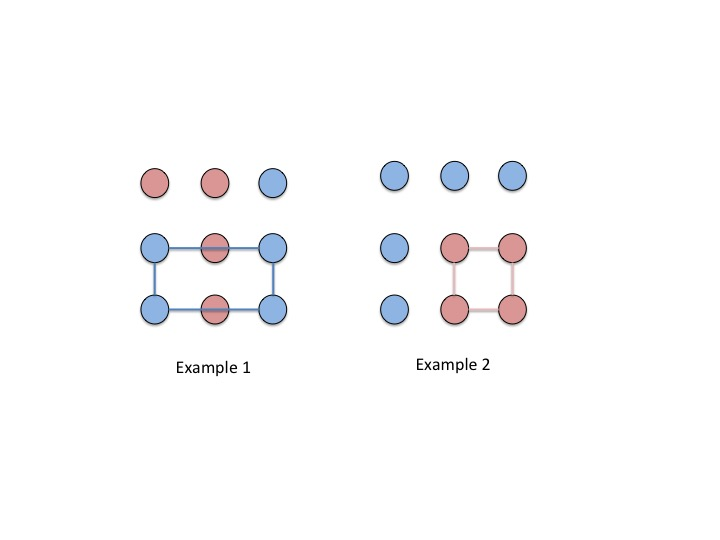
\includegraphics[width=.8\linewidth]{Slide1.jpg}
\end{minipage}

In a 3 x 9 grid there are three dots in each column. Since there are only two colors, red and blue, at least two of the three dots must be the same color (Pigeonhole Principle). Given this restriction there are eight different possible column setups, which can be seen below:

\begin{minipage}{.8\textwidth}
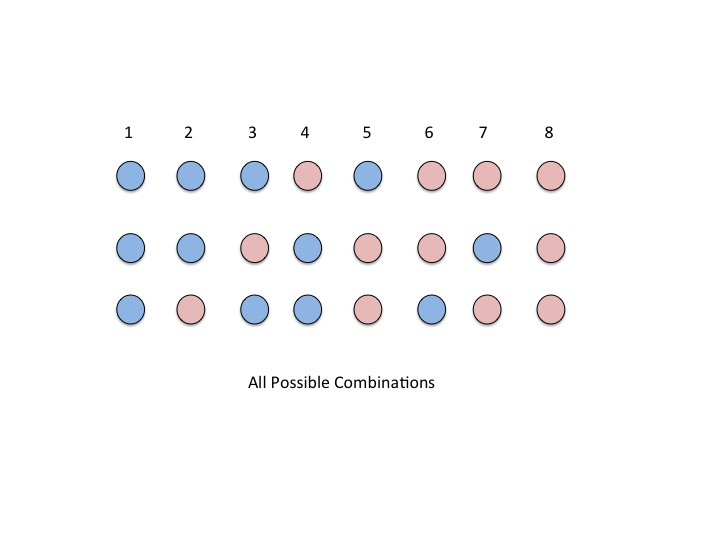
\includegraphics[width=.8\linewidth]{Slide2.jpg}
\end{minipage}

Since there are 9 columns, and 8 possible column formations, one formation must be repeated due to the pigeonhole principle. As shown earlier, this repeated column will form a rectangle with it's duplicate because both columns will have at least two colored points in the same location. Therefore, a 3 x 9 grid must contain a rectangle with four points of the same color. 
\end{proof}

\pagebreak
\section*{Problem Six: Properties of Relations: Katie}

\paragraph{i.} The relation $<$ over the set of real numbers is neither an equivalence relation nor a partial order. A common property of equivalence relations and partial orders is that both must be reflexive. This means that every element is related to itself, or formally, that $\forall a \in A.\ aRa$. However, the relation $<$ over the set of real numbers is not reflexive; by the definition of what it means for one quantity to be ``less than" another, it is not the case that $\forall a \in A.\ a<a$. Thus, the relation $<$ is neither an equivalence relation nor a partial order. 

\paragraph{ii.} A relation that is represented by a graph where all nodes have self-edges and there are no edges between distinct nodes is an example of a relation that is both a partial order and an equivalence relation:

\begin{figure}[h]
\centering
  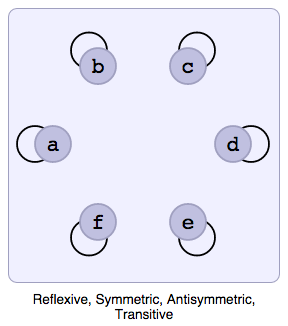
\includegraphics[width=0.45\linewidth]{hw4_6ii.png}
  \caption{A graph where all nodes have self-edges and there are no edges between distinct nodes}
  \label{fig:q6ii}
\end{figure}

In this graph, each node is an element, and an edge from a to b indicates that a is related to b. 

To show that this is a partial order, we show that the relation is reflexive, transitive, and antisymmetric. The relation is reflexive; that is, we drew the graph such that every element is related to itself, or formally, $\forall a \in A.\ aRa$. The relation is transitive; whenever $a$ is related to $b$ and $b$ is related to $c$, we know $a$ is related to $c$, or formally, $\forall a \in A.\ \forall b \in A.\ \forall c \in A.\ (aRb \wedge bRc \rightarrow aRc)$. This is vacuously true, because in the relation we have defined, the antecedent is always false (it is never the case that any element is related to a distinct other object). Finally, the relation is antisymmetric; if $a$ is related to $b$ and $a \neq b$, then $b$ is not related back to $a$, or formally, $\forall a \in A.\ \forall b \in A.\ (a \neq b \wedge aRb \rightarrow \neg(bRa))$. Again, this is vacuously true, because in the relation we have defined, the antecedent is always false (it is never the case that any element is related to a distinct other object).

To show that this is an equivalence relation, we show that the relation is reflexive and transitive (which we have already shown), as well as symmetric. The relation is symmetric; if $a$ is related to $b$, then $b$ is related to $a$, or formally, $\forall a \in A. \forall b \in A.\ (aRb \rightarrow bRa)$. As before, this is vacuously true, because in the relation we have defined, the antecedent is always false (it is never the case that any element is related to a distinct other object).  

The relation we have defined is reflexive, transitive, antisymmetric, and symmetric. Thus, this relation is an example of a relation that is both a partial order and an equivalence relation.

\paragraph{iii.} The relation $=_H$ over P, the set of all people, is an equivalence relation. To show that this is an equivalence relation, we show that $=_H$ is reflexive, transitive, and symmetric. $=_H$ is reflexive; every person is equal in height to themselves, or formally, $\forall p \in P.\ p =_H p$. Next, we show that $=_H$ is transitive; whenever person $p$ is equal in height to person $q$, and person $q$ is equal in height to person $r$, then person $p$ is equal in height to person $r$, or formally, $\forall p \in P.\ \forall q \in P.\ \forall r \in P.\ (p =_H q \wedge q =_H r \rightarrow p =_H r)$. Finally, $=_H$ is symmetric; if person $p$ is equal in height to person $q$, then person $q$ is equal in height to person $p$, or formally, $\forall p \in P. \forall q \in P.\ (p =_H q \rightarrow q =_H p)$. Thus, we have shown that $=_H$ is an equivalence relation.

\paragraph{iv.} The relation $\leq_H$ over P, the set of all people, is not a partial order. To show that this is the case, we show that one of the defining properties of partial orders, antisymmetry, does not hold for the relation $\leq_H$. For a relation to be antisymmetric, it must be the case that:
$$\forall a \in A.\ \forall b \in A.\ (aRb \wedge bRa \rightarrow a=b).$$
Stated in plain English, this says, ``If $a$ is related to $b$ and $b$ is related back to $a$, then $a = b."$ However, we know that this is not the case. There could exist two distinct people, person $p$ and person $q$, where person $p$ is the same height as person $q$. In other words:
$$\exists p \in P.\ \exists q \in P.\ (p \leq_H q \wedge q \leq_H p \wedge p \neq q)$$
This contradicts the property of antisymmetry; we have shown $P \wedge \neg Q$, negating the implication. Because the relation $\leq_H$ is not antisymmetric, we know that it is not a partial order.

\section*{Problem Seven: Meet Semilattices: Marty}

\paragraph{i.} 
\paragraph{ii.}
\paragraph{iii.} 
\begin{thm} The relation $\le_S$ is reflexive. \end{thm}
\begin{proof} 
\end{proof}

\begin{thm} The relation $\le_S$ is transitive. \end{thm}
\begin{proof} A relation is transitive when the following holds: $\forall a \in A .\ \forall b \in A .\ \forall c \in A .\ (aRb \wedge bRc \rightarrow aRc)$. In this case, we want to show that $\forall x \in D .\ \forall y \in D .\ \forall z \in D .\ (x \le_S y \wedge y \le_S z \rightarrow x \le_S z)$. To prove this, we assume that the antecedent is true and show that the consequent must be true as well. We have that both $x \le_S y$ and $y \le_S z$. From the definition of $\le_S$ we know that $x \wedge y = x$ and $y \wedge z = y$. Combining these gives us $x \wedge y \wedge z = x$. 
\begin{align*}
x \wedge y \wedge z &= x
x \wedge z &= z
\end{align*}
We have shown that when we assume the antecendent, the consequent is true. This proves that $\le_S$ is transitive.
\end{proof}

\begin{thm} The relation $\le_S$ is antisymmetric. \end{thm}
\begin{proof} A relation is antisymmetric when the following holds: $\forall a \in A .\ \forall b \in A .\ (aRb \wedge bRa \rightarrow a = b)$. In this case, we want to show that $\forall x \in D .\ \forall y \in D .\ (x \le_S y \wedge y \le_S x \rightarrow x = y)$. To prove this, we assume that the antecedent is true and show that the consequent must be true as well. We have that both $x \le_S y$ and $y \le_S x$. From the definition of $\le_S$ we know that $x \wedge y = x$ and $y \wedge x = y$. From the commutative property of the meet semilattice we know that $y \wedge x = x \wedge y = y$. Because $x \wedge y = x$ and $x \wedge y = y$, we know that $x = y$. We have shown that when we assume the antecedent, the consequent must be true. This proves that $\le_S$ is antisymmetric.
\end{proof}

\paragraph{iv.}
\paragraph{v.}

\section*{Problem Eight: Chains and Antichains: Katie}

\paragraph{i.} The longest chain in the partial order of the $\subeq$ relation over the set $\wq(\{a, b, c\})$ has a length of 4. An example of such a chain:
$$\emptyset \subeq \{a\} \subeq \{a, b\} \subeq \{a, b, c\}$$

\paragraph{ii.}
\paragraph{iii.}
\paragraph{iv.}

% \section*{Appendix: Referencing Equations}
% \begin{equation} \label{eq:divbyzero}
%   \frac {1} {0}
% \end{equation}

% This references \ref{eq:divbyzero}.

% \section*{Appendix: Figures in Text}
% Below are two different ways of placing figures side by side in text. The first method creates two sub-figures within a single figure. The second method creates two separate figures.

% \begin{figure}
% \centering
% \begin{minipage}{.5\textwidth}
%   \centering
%   \includegraphics[width=.8\linewidth]{hw3_8_1.eps}
%   \captionof{figure}{A figure}
%   \label{fig:q8_test1}
% \end{minipage}%
% \begin{minipage}{.5\textwidth}
%   \centering
%   \includegraphics[width=.8\linewidth]{hw3_8_1.eps}
%   \captionof{figure}{Another figure}
%   \label{fig:q8_test2}
% \end{minipage}
% \end{figure}


% \begin{figure}[h]
%   \centering

%   \begin{subfigure}[b]{0.3\textwidth}
%     \includegraphics[width=\textwidth]{hw3_8_1.eps}
%     \caption{A cycle with length $k+1$}
%     \label{fig:q8_cycle:a}
%   \end{subfigure}% 
%   \qquad
%   \begin{subfigure}[b]{0.3\textwidth}
%     \includegraphics[width=\textwidth]{hw3_8_1.eps}
%     \caption{A cycle with length $k+1$}
%     \label{fig:q8_cycle:b}
%   \end{subfigure}%  

%   \caption{Placeholder}
%   \label{fig:q8}
% \end{figure}

\end{document}
	% line of code telling latex that your document is ending. If you leave this out, you'll get an error

%%% Local Variables:
%%% mode: latex
%%% TeX-master: t
%%% End:
